\documentclass[a4paper, 12pt]{article}
\usepackage[utf8]{inputenc}
\usepackage{amsmath}
\usepackage{graphicx}
\usepackage{fancyhdr}
\usepackage{imakeidx}
\usepackage[]{algorithm2e}

\title{
\textbf{Metaheurística - Práctica 1.a} \\
Técnicas de Búsqueda Local y Algoritmos Greedy para el Problema de la Asignación Cuadrática
}

\author{
3º Grado Ingeniería Informática, Grupo 3 (Miércoles)\\
Salvador Corts Sánchez, 75935233C \\
salvacorts@correo.ugr.es
}

\date{}

\fancyhead[LE,RO]{Salvador Corts Sánchez, 75935233C}
\fancyhead[RE,LO]{QAP: Práctica 1}
\pagestyle{fancy}

\makeindex

\begin{document}
   % Header
   \maketitle
   
   % Index
   \newpage
   \tableofcontents

   
   % Descripción del problema
   \newpage
   \section{Descripción del problema}
   El problema de asignación cuadrática (en inglés, quadratic assignment problem, QAP) es uno de los problemas de optimización combinatoria más conocidos. En él se dispone de n unidades y n localizaciones en las que situarlas, por lo que el problema consiste en encontrar la asignación óptima de cada unidad a una localización. La nomenclatura “cuadrático” proviene de la función objetivo que mide la bondad de una asignación, la cual considera el producto de dos términos, la distancia entre cada par de localizaciones y el flujo que circula entre cada par de unidades. El QAP se puede formular como:
   
   $$QAP = 
\begin{matrix}
min\\
\pi \in \prod_N 
\end{matrix}   \Bigg( \sum_{i=1}^{n} \sum_{j=1}^{n} f_{ij}d_{\pi(i)\pi(j)} \Bigg)   
   $$
   
   donde:
   \begin{itemize}
      \item \textbf{$\pi$} es una solución al problema que consiste en una permutación que representa la asignación de la unidad $i$ a la localización  $\pi(i)$.
      
      \item $f_{ij}$ es el flujo que circula entre la unidad $i$ y la $j$.
      
      \item $d_{kl}$ es la distancia existente entre la localización $k$ y la $l$.
   \end{itemize}
   
   
   % Descripción de la aplicación de los algoritmos
   \newpage
   \section{Consideraciones comunes a los algoritmos utilizados}
   Esta práctica ha sido diseñada como una librería de metaheurísticas per se. Es decir, existe un tipo de objeto \textbf{Solution} y un tipo de objeto \textbf{Solver} del cual heredarán los objetos que implementan las diversas metaheurísticas. Cada metaheurística deberá implementar la función \textit{Solve} que devuelve un objeto \textbf{Solution}.
   
   \subsection*{Clase Solver}
   Esta clase debe ser heredada por las metaheurísticas a implementar. Su representación consta de dos matrices:
   \begin{itemize}
      \item \textbf{Distancias}: Matriz de distancias entre un punto $i$ y otro $j$.
      \item \textbf{Frecuencias}: Matriz de flujo entre un objeto $i$ y otro $j$. 
   \end{itemize}
   Tiene una función virtual llamada \textit{Solve} que ha de ser implementada por los objetos que hereden de \textbf{Solver}. Es la interfaz común a todos los objetos de tipo Solver para obtener una Solución.
   
   \newpage
   \subsection*{Clase Solution}
   Sirve para representar una solución, la cual, se implementa como un vector donde cada posición $i$ representa un objeto y alberga la localización $j$ donde debe ser colocado dicho objeto $i$. 
   
   \begin{center}
      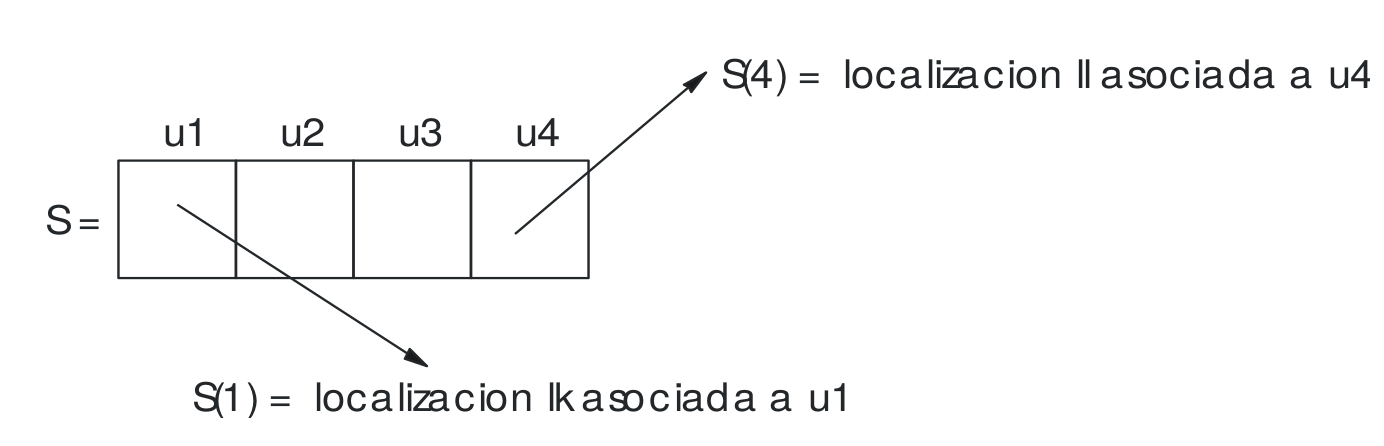
\includegraphics[scale=0.14]{solRep}
   \end{center}
   
   Existe una función \textit{CalcCost} que calcula el coste de dicha solución como:
      $$cost = \sum_{i=1}^{n}\sum_{j=1, j \neq i}^{n} f_{ij}d_{\pi(i)\pi(j)}$$
   donde:
   \begin{itemize}
      \item $\pi$ es la solución al problema.
      
      \item $f_{ij}$ es el flujo que circula entre la unidad $i$ y la $j$.
      
      \item $d_{kl}$ es la distancia existente entre la localización $k$ y la $l$.
   \end{itemize}\vspace*{0.5cm}
   
   Dado que el cálculo del coste de la solución es bastante costoso, $O(n^{2})$, Esta función debe llamarse manualmente al menos una vez para obtener el coste y que este se guarde en la representación de la clase.
   
   
   \newpage
   \section{Algoritmo Greedy}
   Se basa en el cálculo de los potenciales de flujo y distancia definidos como:
   \begin{center}
      $\hat{f}_i = \sum_{j=1}^{n}f_{ij}$ \hspace*{1cm} $\hat{d}_i = \sum_{j=1}^{n}d_{ij}$
   \end{center}
   
   El algoritmo irá seleccionando la unidad $i$ libre con mayor $\hat{f}_i$ y le asignará la localización $j$ libre con menor $\hat{d}_j$. Su implementación en pseudocódigo es la siguiente:  
      \begin{algorithm}
          \# Calcula los potenciales\\
          $dp = fp = vector(n)$\\
          \For{$i=0$ \KwTo $n$}{
             $\hat{f}_i = \hat{d}_i = 0$\\
             \For{$j=0$ \KwTo $n$}{
                $\hat{f}_i = \hat{f}_i + f_{ij}$\\
                $\hat{d}_i = \hat{d}_i + d_{ij}$\\
             }
             $dp_i = \hat{d}_i$\\
             $fp_i = \hat{f}_i$\\
          }\vspace*{0.5cm}
          
          \# Calcula la mejor combinación. $\pi$ es la representación de la solución\\
          $locAssigned = unitAssigned = vector(n)\{0\}$\\
          \For{$i=0$ \KwTo $n$}{
             $best\hat{f} = -\infty$;\hspace*{0.5cm}$best\hat{f}_{index}=0$\\
             $best\hat{d} = \infty$;\hspace*{0.5cm}$best\hat{d}_{index}=0$\\
             \For{$j=0$ \KwTo $n$}{
                $\hat{f}_i = fp_j$;\hspace*{0.5cm}$\hat{d}_i = dp_j$\\
                
                \If{$\hat{f}_i > best\hat{f}$ \textbf{and} $unitAssigned_j \neq 1$}{
                   $best\hat{f} = \hat{f}_i$;\hspace*{0.5cm}$best\hat{f}_{index}=j$\\
                }
                
                \If{$\hat{d}_i < best\hat{d}$  \textbf{and} $locAssigned_j \neq 1$}{
                   $best\hat{d} = \hat{d}_i$;\hspace*{0.5cm}$best\hat{d}_{index}=j$\\
                }
             }
             $\pi(best\hat{f}_{index}) = best\hat{d}_{index}$\\
             $unitAssigned_{best\hat{f}_{index}} = locAssigned_{best\hat{d}_{index}} = 1$\\             
          }
      \end{algorithm}
      
      
      \newpage
      \section{Algoritmo de Búsqueda Local}
      Vamos a utilizar una \textbf{búsqueda local del primer mejor}. Cuando se genera una solución vecina que mejora a la actual, se toma esta como solución y se pasa a la siguiente iteración. Se detiene la búsqueda cuando no se genera ningún vecino mejor que la solución actual.\\
      
      Como se comentó anteriormente, el proceso de cálculo del coste de la solución es de orden cuadrático por lo que realizar dicho calculo con cada vecino es sumamente costoso; En su lugar, vamos a considerar una \textbf{factorización} teniendo en cuenta solo los cambios realizados por el movimiento de intercambio para generar el vecino.
      
      
      \subsection*{Búsqueda Local con \textit{Don't Look Bits}}
      b\\
   
\printindex
\end{document}
